
%\documentstyle[epsf,twocolumn]{jarticle}       %LaTeX2e仕様
\documentclass[twocolumn]{jarticle}     %pLaTeX2e仕様(platex.exeの場合)
% \documentclass[onecolumn]{ujarticle}   %pLaTeX2e仕様(uplatex.exeの場合)
%%%%%%%%%%%%%%%%%%%%%%%%%%%%%%%%%%%%%%%%%%%%%%%%%%%%%%%%%%%%%%
%%
%%  基本バージョン
%%
%%%%%%%%%%%%%%%%%%%%%%%%%%%%%%%%%%%%%%%%%%%%%%%%%%%%%%%%%%%%%%%%
\setlength{\topmargin}{-45pt}
%\setlength{\oddsidemargin}{0cm}
\setlength{\oddsidemargin}{-7.5mm}
%\setlength{\evensidemargin}{0cm}
\setlength{\textheight}{24.1cm}
%setlength{\textheight}{25cm}
\setlength{\textwidth}{17.4cm}
%\setlength{\textwidth}{172mm}
\setlength{\columnsep}{11mm}

%\kanjiskip=.07zw plus.5pt minus.5pt


% 【節が変わるごとに (1.1)(1.2) … (2.1)(2.2) と数式番号をつけるとき】
%\makeatletter
%\renewcommand{\theequation}{%
%\thesection.\arabic{equation}} %\@addtoreset{equation}{section}
%\makeatother

%\renewcommand{\arraystretch}{0.95} 行間の設定
%%%%%%%%%%%%%%%%%%%%%%%%%%%%%%%%%%%%%%%%%%%%%%%%%%%%%%%%
%\usepackage{graphicx}   %pLaTeX2e仕様(\documentstyle ->\documentclass)
\usepackage[dvipdfmx]{graphicx}
\usepackage{subcaption}
\usepackage{multirow}
\usepackage{amsmath}
\usepackage{url}
\usepackage{ulem}
\usepackage{algorithm}
\usepackage{algorithmic}
\usepackage{listings} %,jlisting} %日本語のコメントアウトをする場合jlistingが必要
%ここからソースコードの表示に関する設定
\lstset{
  basicstyle={\ttfamily},
  identifierstyle={\small},
  commentstyle={\smallitshape},
  keywordstyle={\small\bfseries},
  ndkeywordstyle={\small},
  stringstyle={\small\ttfamily},
  frame={tb},
  breaklines=true,
  columns=[l]{fullflexible},
  numbers=left,
  xrightmargin=0zw,
  xleftmargin=3zw,
  numberstyle={\scriptsize},
  stepnumber=1,
  numbersep=1zw,
  lineskip=-0.5ex
}
\newcommand{\argmax}{\mathop{\rm arg~max}\limits}
\newcommand{\argmin}{\mathop{\rm arg~min}\limits}

%%%%%%%%%%%%%%%%%%%%%%%%%%%%%%%%%%%%%%%%%%%%%%%%%%%%%%%%
\begin{document}

	%bibtex用の設定
	%\bibliographystyle{ujarticle}

	\twocolumn[
		\noindent
		\hspace{1em}
		2021 年 6 月 28 日
		発表資料
		\hfill
		M1 杉山 竜弥
		\vspace{2mm}

		\hrule
		\begin{center}
			{\Large \bf 仮タイトル}
		\end{center}
		\hrule
		\vspace{9mm}
	]

\section{はじめに}

% 実データとボットの識別.
% (識別機で生成の評価ができる)

自然言語分野では, 文章生成など創作に関わるものも人間と遜色なく生成できるようになり,
大きく注目されている.

人の考えた文章と計算機が生成した文章との違いに注目した.


本研究では
オープンソース化されていないGPT-3に代わって,
前身のGPT-2を使って, 文章の破綻推定をした.
人工知能に人の文章と自動生成の文章が識別できるのかと,
GPT-2の文章生成能力の確認実験をした.

\section{要素技術}
\subsection{Transformer}
Transformer\cite{DBLP:journals/corr/VaswaniSPUJGKP17} は再帰的ニューラルネットワーク (Recurrent Neural Network: RNN)\cite{mikolov2010recurrent} を使わずに, Self-Attention を使って並列計算を可能にするモデルである.

RNN は時系列に沿って順番に計算する構造であるため並列計算ができず,
GPU などを使っても計算時間が長いという欠点がある.
GPU の性能を十分に活用し, 計算速度を向上させるため, RNN を使用しないことが必要となる.

% Self-Attentionとは、attentionの実践のところで紹介しましたが、もともとの論文にあった 翻訳語の単語から翻訳前の単語に注意を向けるattentionではなく、自分自身のどこが重要かに注意を向ける.
Self-Attentionは, シーケンス内の単語間の関係性に注目する.
TransformerはSelf-Attentionの計算を並列化するとこで効率的な計算ができる.

% Positional Encoding



\begin{figure}[tb]
  \begin{center}
    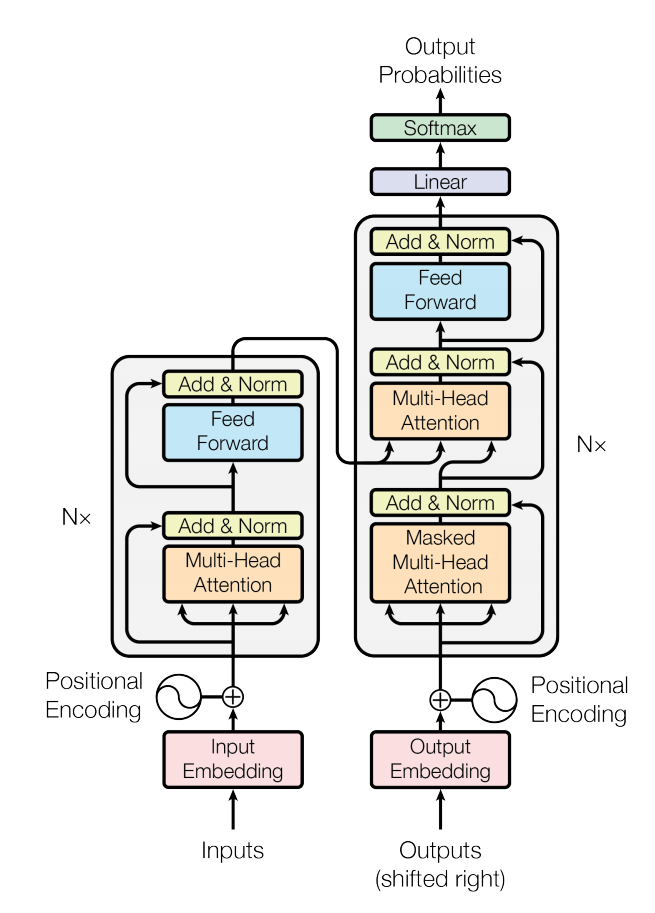
\includegraphics[clip,width=75mm]{Transformer.png}
    \caption{Transformer}
    \label{fig:trans}
  \end{center}
\end{figure}



\subsection{GPT-2}
Generative Pretrained Transformer 2 (GPT-2)\cite{radford2019language} は

特定のタスクに特化した数万の教師ありデータでファインチューニングが必要だった GPT, BERT をはじめとしたモデルと異なり,
Transformerのデコーダ部分を利用し,
大規模な言語コーパスで様々なタスクを学習する汎用的なモデルとして設計された.

任意の長さの文章をシンボルにしたシーケンスを $(s_1, s_2, ..., s_n)$ とする.
同時確率は条件付確率の積に分解される.
\begin{equation}
p(x) = \prod^n_{i=1} p(s_n|s_1, ... , s_{n-1})
\end{equation}
この条件付確率は, Transformer\cite{DBLP:journals/corr/VaswaniSPUJGKP17}によって効率的に計算できる.

GPT-2では, $p(\mathrm{output} | \mathrm{input})$ を一般化して,
$p(\mathrm{output} | \mathrm{input}, \mathrm{task})$と表しタスクの種類も学習することで, 特定の問題のためのファインチューニングなしで, 1つのモデルでも問題を解けるようにしている.


\begin{table}[tbh]
  \begin{center}
    \caption{GPT-2の解けるタスク}
    \begin{tabular}{|c|} \hline
      AutomaticSpeechRecognition \\ \hline
      Conversational \\ \hline
      FeatureExtraction \\ \hline
      FillMask \\ \hline
      ImageClassification \\ \hline
      QuestionAnswering \\ \hline
      Summarization \\ \hline
      TextClassification \\ \hline
      TextGeneration \\ \hline
      TokenClassification \\ \hline
      Translation \\ \hline
      ZeroShotClassification \\ \hline
      % Text2TextGeneration \\ \hline
      % TableQuestionAnswering \\ \hline
    \end{tabular}
    \label{tab:task}
  \end{center}
\end{table}

\subsection{Byte Pair Encoding}
Byte Pair Encoding (BPE) は高頻度の単語は単語全体を辞書に登録し、低頻度の単語は文字単位に分割する言語モデルにおける未知語処理手法である.

言語モデルは語彙サイズをハイパーパラメータとして設定するため, ニューラルモデルに扱われない未知語が存在する.
未知語処理として, $<unk>$ などの特殊トークンに置き換える方法と, 単語をより細かく分割しサブワードにすることで語彙を少なくする方法がある.

BPE は
データ圧縮手法を言語モデルに応用した.
文字単位に単語を分解し, 2 文字のペアの中で高頻度の要素を結合して 1 つのサブワードとする手順を繰り返すことで,
単語を接頭辞や接尾辞などの意味のある単位に分解できる.

\subsection{Manga 109}
Manga 109 \cite{mtap_matsui_2017} は, 漫画の学術研究への使用を目的と
して作成された研究用コミックデータセットである.
1970 年代から 2010 年代に公開された, 日本のプロ
漫画家によって描かれた漫画 109 冊で構成されて
いる.


\subsection{BERT}
BERT \cite{devlin2018bert} は, 2018 年に Google が発表した汎用言語モデルである.
複数の双方向 Transformer を用いることで文脈を考慮することができるモデルとされている.
各タスクに対してファインチューニングをすることでさまざまなタスクに柔軟に対応することができる.

事前学習には入力の一部の単語を “[MASK]” に置き換えてその元単語を予測するように訓練するタスク (Masked Language Model) と 2 文を入力としてその連続性を識別するように訓練するタスク (Next Sentence Prediction) が用意されている.
% 本研究の実験では,  東北大学によって公開されている BERT 日本語 Pretrained モデルを使用した.
本研究では, 入力する文章の分類器として選んだ.


\section{提案手法}

\begin{table}[tb]
  \begin{center}
    \caption{GPT-2 の設定}
    \begin{tabular}{cc}
      \hline
      parameter & value \\
      \hline
      max length & 50 \\
      top p & 0.95 \\
      top k & 60 \\
      \hline
    \end{tabular}
    \label{tab:setting_gpt}
  \end{center}
\end{table}

\begin{table}[tb]
  \begin{center}
    \caption{BERT の設定}
    \begin{tabular}{cc}
      \hline
      parameter & value \\
      \hline
      Optimizer & AdamW \\
      lr & 2e-5 \\
      loss & Cross Entropy \\
      batch size & 32 \\
      train data & 12502 \\
      valid data & 1389 \\
      test data & 1543 \\
      epoch & 20 \\
      \hline
    \end{tabular}
    \label{tab:setting_bert}
  \end{center}
\end{table}


\begin{table*}[tb]
  \begin{center}
    \caption{GPT-2 の生成した文章の例}
    \begin{tabular}{ccc}
    \hline
    \textbf{title}                     & \multicolumn{2}{c}{\textbf{sentence}}      \\
    \hline
    \multirow{3}{*}{Akuhamu}           & $S_i$    & 我 梢つつじの名において命じる!                 \\
                                       & $S_{i+1}$  & いでよ! 悪魔っ                         \\
                                       & $S'_{i+1}$ & あなたは、我 の の は を どうする ら れ ば いいのですか \\
    \multirow{3}{*}{YouchienBoueigumi} & $S_i$    & 最近世間がぶっそうだわ                      \\
                                       & $S_{i+1}$  & いつまでも人任せに安穏としていていいのかしら…          \\
     & $S'_{i+1}$ & \small{\begin{tabular}[c]{@{}c@{}}・ ・ ・ ・ なんでこういうことになったのか知らないが、今から思えば大問題 ・ ・ ・ \\ こういうことをやっている人には何を言っても無駄なのか\end{tabular}}\\
     \hline
     \multicolumn{3}{l}{©あくはむ 新居 さとし,   ©幼稚園ぼうえい組 テンヤ}
    \end{tabular}
    \label{tab:gpt_gen}
  \end{center}
\end{table*}


人間が作成した文章と, GPT-2が作成した文章のデータセットを作成し,
BERTで作成者を推定する問題を解く.

\subsection{データセット}
人間が作成した文章として Manga 109 中のセリフを利用した.


~~~として, 連続する 2 文をつかう.

文章間の意味が繋がっている必要があるが, 意味を考慮した単位に文章を分割するのは難しい.
そのため決められたフォーマットで, 繋がりを持った文章として仮定しやすい 4 コマ漫画を対象として
Manga109 中の 5 作品のデータを用いた.

% データの構造

Manga109 のセリフデータを $S_1$, $S_2$, $S_n$ として, 連続する 2 文を実際のデータ,GPT-2 で次の文章を推測した $S’$ を含んだ 2 文を生成データとして, データセットを作成した.
文と文の間は [SEP] トークンで結合しました.

GPT-2 による生成では, 生成文の句点までを 1 文とし, [SEP], [EOS] などのトークンは削除したものを $S’$ とした.


\subsection{分類問題}
実データのラベルを 1, 生成データのラベルを 0として BERTを利用して 2値分類問題を解く.

高いとBERTで分類可能性.
低いとGPT-2の文章生成能力が高い.

% \subsection{対話タスク}
%
% 図 \ref{fig:con} に対話例を示した.
% 英語の場合, 対話を自然に続けられることを確認した.
%
% \begin{figure}[tb]
%   \begin{center}
%     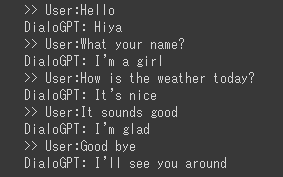
\includegraphics[clip,width=75mm]{ss.png}
%     \caption{対話例}
%     \label{fig:con}
%   \end{center}
% \end{figure}

\section{実験}

表 \ref{tab:setting_gpt}, 表 \ref{tab:setting_bert} は GPT-2 と BERT の実験パラメータである.
GPT-2 の事前学習パラメータにはrinna/japanese-gpt2-mediumを, BERTの事前学習パラメータには東北大学が公開するモデルを使用した.


\subsection{生成の結果}

表 \ref{tab:gpt_gen} に GPT-2 による生成結果の例を示す.
この結果より, BERT の学習するデータセットを作成した.

% 考察
生成されたデータには漫画的特徴よりも, 事前学習に含まれていたと思われる ブログ, 掲示板, 小説, SNS などの表現が多く生成されていた.
表 \ref{tab:gpt_gen} のように漫画のセリフとしては, コマに入らないような比較的長い文章が生成される傾向にあった.

本実験では入力するプロンプトとして 1 文のみを入力したが, より前の文章も与えることで漫画の特徴を掴んだ文章生成ができることが考えられる.



% 漫画のセリフよりも長い文章が生成されている.

\subsection{分類の結果}

\begin{table}[tb]
  \begin{center}
    \caption{分類実験の結果}
    \begin{tabular}{ccc}
      \hline
       & loss & accuracy \\
      \hline
      train & 0.010 & 0.997 \\
      test & 0.123 & 0.959 \\
      baseline & --- & 0.50 \\
      \hline
    \end{tabular}
    \label{tab:result}
  \end{center}
\end{table}

\begin{table}[tb]
  \begin{center}
    \caption{混合行列}
    \begin{tabular}{|c|c|c|c|}
    \hline
    \multicolumn{2}{|c|}{\multirow{2}{*}{\textbf{}}} & \multicolumn{2}{c|}{予測} \\ \cline{3-4}
    \multicolumn{2}{|c|}{}                           & 1               & 0              \\ \hline
    \multirow{2}{*}{ラベル}              & 1             & 753              & 39              \\ \cline{2-4}
                                     & 0             & 25              & 726             \\ \hline
    \end{tabular}
    \label{tab:conmat}
  \end{center}
\end{table}


\begin{table*}[tb]
  \begin{center}
    \caption{BERT の誤識別例}
    \begin{tabular}{ccc}
      \hline
      input & label & pred \\
      \hline
      \verb|[CLS]極道をやっとりましたが足を洗い[SEP]ホストクラブや寿司屋で働いてましたが[EOS]| & 1 & 0 \\
      \verb|[CLS]というふうに去年は笑ってられたけど[SEP]今年はそうもいきませんね[EOS]| & 1 & 0 \\
      \verb|[CLS]いつもどったんですか!?[SEP]よっ[EOS]| & 1 & 0 \\
      \verb|[CLS]ふふん[SEP]正しいんだけど何かちがう気がする……[EOS]| & 1 & 0 \\
      \verb|[CLS]大き・・さ・・など関・・・係・・・ない[SEP]・・事・・・だと言う事・・・[EOS]| & 0 & 1 \\
      \verb|[CLS]立ちどまってもくれない[SEP]いや 立とうともしない[EOS]| & 0 & 1 \\
      \verb|[CLS]極道の生態に親しむこのツアー[SEP]も4年目になる[EOS]| & 0 & 1 \\
      \verb|[CLS]子供の頃から普通の男にはなるなと[SEP]先生に言われていた[EOS]| & 0 & 1 \\
      \hline
      \multicolumn{3}{l}{©徹さん	川口 憲吾,   ©OLランチ	さんり ようこ,  ©高校の人達	葛原 兄}
    \end{tabular}
    \label{tab:bert_result}
  \end{center}
\end{table*}

表 \ref{tab:result} は BERT による分類の学習結果を示す.
2 値分類であるため正答率のベースラインは 0.5 であるが, テストデータで 0.959 という高い精度で分類できたと言える.
この結果は BERT の文章の識別問題への有効性を示すとともに, 本実験設定でのGPT-2 と人間による文章との間には大きな違いがあることを示唆している.

% 0.997280	0.009569
% test loss:  0.12322708242572844  test acc:  0.9585223590408296

% 考察.

表 \ref{tab:conmat} は分類結果の混合行列,
表 \ref{tab:bert_result} は BERT の分類の誤りの例である.
表 \ref{tab:conmat} の結果から, 人間の文章を GPT-2 の文章と誤っている回数が多いことが分かる.

表 \ref{tab:bert_result} の label=1, pred=0 となっている部分を見ると,
[SEP] トークンを挟んで文章が続いているパターンがあった.
GPT-2 の生成した文章に頻繁にあるパターンであるため, 誤って識別したと考えられる.
また 2 文のうち 1 方が, 呼びかけなどで短すぎる場合もあり, この情報だけで判断するのは人間とっても困難であると思われる.

反対に GPT-2 の文章を人間の文章と誤っている例を見ると,
文脈の短さも相まって一見自然な文章が生成されていると感じられた.
特に最初の例では, 時間的空白を表す文字が挟まっているにも関わらず, 文体の特徴を捉えながら意味のつながった文章が出力されている.
この例から考えると, GPT-2 でも一部自然な文章が生成できているということが確認できた.

\section{まとめと今後の課題}

% まとめ
本研究では人の考えた文章と GPT-2 が生成した文章との違いに注目し,
人間と比較して GPT-2 が生成した文章の自然さの確認を実験した.
文章の比較に BERT を利用して識別タスクを学習した.

結果 BERT は高い精度で人間と GPT-2 の文章を見分けることができるということがわかった.
一方でこの識別に関してはデータセットに使用した漫画という媒体が持つ特有の文章形式と GPT-2 の学習したデータの違いが識別に少なくない影響があったと考えられる.
また GPT-2 の文章を人間の文章と誤っている例から GPT-2 が一部自然な文章生成ができることも確認できた.


% 課題.
今後の課題としては, GPT-3 を利用して同様の実験をし性能を比較することが挙げられる.
またGPT-2 に与える入力文章を長くすることによって, GPT-2 がより自然な文章を出力できるようになる可能性もあるため, GPT-2 の設定を見直したい.

% 参考文献リスト
\bibliographystyle{unsrt}
\bibliography{ref}
\end{document}
